\chapter{DESENVOLVIMENTO}

O desenvolvimento experimental deste trabalho foi organizado em etapas complementares, com o propósito de avaliar o custo computacional da aplicação de algoritmos criptográficos a mensagens de barramento CAN. Inicialmente, foi implementado um programa de \textit{benchmark} em linguagem C, utilizando a biblioteca OpenSSL para processar dados extraídos de um conjunto público de mensagens CAN. Posteriormente, os resultados das execuções foram organizados e analisados por meio de um \textit{script} em Python, responsável pelo cálculo de estatísticas descritivas e pela elaboração dos gráficos comparativos.

O programa em C realiza a leitura dos registros do conjunto de dados, extrai o conteúdo útil das mensagens e o converte em estruturas adequadas ao processamento criptográfico. Sobre essas entradas, são executadas operações com AES-128, ChaCha20, RSA e uma construção demonstrativa baseada em criptografia de curvas elípticas (ECC), denominada ECIES-P256. Diferentemente dos demais algoritmos, a ECC não representa um algoritmo específico de cifragem, mas uma abordagem criptográfica baseada em operações matemáticas sobre curvas elípticas. Por esse motivo, foi utilizada uma implementação demonstrativa inspirada no Elliptic Curve Integrated Encryption Scheme (ECIES), empregando a curva P-256 para realizar o estabelecimento de um segredo compartilhado por meio do protocolo ECDH, posteriormente utilizado na derivação de uma chave simétrica para a cifragem dos dados. Dessa forma, o ECIES-P256 permite representar a aplicação prática da criptografia baseada em curvas elípticas na comparação experimental, embora seu desempenho corresponda ao conjunto de operações da construção implementada, e não exclusivamente às operações matemáticas da ECC. Os experimentos são repetidos em 100 rodadas por algoritmo, permitindo registrar as medidas de desempenho e examinar a variação entre as execuções.

Os dados produzidos são armazenados em arquivos no formato CSV e posteriormente processados em Python. A análise considera a latência de cifragem como métrica principal, complementada pelo \textit{throughput}, pelo uso de memória RAM e pelo tempo de geração de chaves, quando aplicável. A Figura~\ref{fig:fluxograma_benchmark} apresenta o fluxo geral de processamento, desde a entrada das mensagens CAN até a obtenção das tabelas e dos gráficos utilizados na comparação dos algoritmos.

\section{Desenvolvimento do Benchmark em C}

A primeira etapa experimental deste trabalho consistiu no desenvolvimento de um programa em linguagem C, utilizando a biblioteca OpenSSL, com o objetivo de avaliar o desempenho de diferentes mecanismos criptográficos aplicados a dados provenientes de mensagens do barramento CAN. Essa implementação foi utilizada como base para a coleta das métricas de desempenho, permitindo observar o comportamento dos algoritmos em um ambiente computacional controlado.

O programa foi executado em um computador convencional, utilizando o sistema operacional Windows. A escolha da linguagem C ocorreu principalmente pela possibilidade de trabalhar diretamente com sequências de bytes, estruturas de memória e funções disponibilizadas pela biblioteca OpenSSL. Além disso, a linguagem permite organizar as operações criptográficas em rotinas específicas e utilizar recursos do próprio sistema operacional para realizar medições de tempo e consumo de memória.

Para representar os dados utilizados em uma comunicação automotiva, foi empregado um conjunto público de mensagens CAN disponibilizado pelo \textit{Hacking and Countermeasure Research Lab} (HCRL), por meio do \textit{Car-Hacking Dataset}. O conjunto de dados pode ser encontrado no endereço eletrônico \url{https://ocslab.hksecurity.net/}. Nos experimentos, foi utilizado o arquivo \texttt{normal\_run\_data.txt}, contendo registros de tráfego coletados em ambiente automotivo.

A utilização desse conjunto de dados permitiu trabalhar com mensagens provenientes de um contexto real de comunicação veicular, sem a necessidade de manter um veículo conectado durante a execução do programa. Dessa maneira, os testes puderam ser repetidos utilizando uma mesma fonte de dados, reduzindo a influência de alterações que poderiam ocorrer caso as mensagens fossem obtidas continuamente de um barramento em funcionamento.

É importante destacar que o conjunto de dados foi utilizado como fonte de entrada para as operações criptográficas, não sendo realizada uma análise do significado físico das informações presentes nas mensagens. Portanto, valores associados ao funcionamento do veículo, como velocidade, temperatura ou rotação do motor, não foram utilizados como parâmetros para a avaliação dos algoritmos. O interesse do experimento estava concentrado na quantidade de dados processada e no tempo necessário para executar as operações criptográficas.

O funcionamento do programa começa com a abertura e leitura do arquivo contendo os registros CAN. Durante essa etapa, as mensagens são identificadas e seus campos de dados são extraídos para posterior processamento. Como as funções criptográficas trabalham com sequências de bytes, foi necessário preparar as informações extraídas em um formato compatível com as rotinas disponibilizadas pela OpenSSL.

Essa preparação é importante porque os registros armazenados no arquivo possuem uma representação textual, enquanto as operações de cifragem são realizadas sobre dados binários. Assim, o programa realiza a conversão das informações necessárias antes de encaminhá-las aos mecanismos criptográficos. Esse procedimento também permite manter uma estrutura de entrada semelhante entre os algoritmos, respeitando as particularidades de cada implementação.

Após a preparação dos dados, o programa realiza as operações criptográficas utilizando AES-128-CTR, ChaCha20, RSA-2048-OAEP e ECIES-P256. Cada mecanismo possui uma rotina específica, responsável pela preparação dos parâmetros necessários, pela execução da operação e pelo registro das informações utilizadas na avaliação de desempenho.

A separação dessas rotinas foi adotada para facilitar a organização do código e permitir que os mecanismos fossem executados individualmente. Dessa forma, a implementação evita concentrar todas as operações em uma única função, tornando mais simples identificar as etapas responsáveis pelo processamento dos dados e pela coleta das medições.

Embora os quatro mecanismos sejam utilizados no mesmo programa, suas características de funcionamento são diferentes. Por esse motivo, a implementação considera as necessidades específicas de cada rotina, principalmente em relação ao gerenciamento de chaves, aos parâmetros criptográficos e ao tamanho dos dados produzidos. Essas diferenças são relevantes para a organização dos testes e precisam ser consideradas posteriormente na interpretação dos resultados.

Para realizar a avaliação temporal, foi utilizado o recurso \texttt{QueryPerformanceCounter}, disponibilizado pelo sistema operacional Windows. Essa função permite obter valores de um contador de alta resolução, que podem ser utilizados para determinar o intervalo decorrido entre dois instantes. A frequência desse contador é obtida por meio da função \texttt{QueryPerformanceFrequency}, permitindo converter a diferença registrada para uma unidade de tempo.

Durante a execução do benchmark, o programa registra os instantes associados à região de processamento definida para cada algoritmo. A diferença entre esses registros permite calcular a latência da operação, considerada a principal métrica deste trabalho. Essa escolha está relacionada às características das mensagens CAN, que normalmente possuem cargas úteis reduzidas e podem ser transmitidas em intervalos curtos.

Além da latência, o programa também coleta informações relacionadas ao throughput, ao consumo de memória RAM e ao tempo de geração de chaves, quando aplicável. O throughput é utilizado como uma medida complementar da quantidade de dados processada em determinado intervalo, enquanto o consumo de memória permite observar os recursos utilizados durante a execução dos mecanismos criptográficos.

Para a obtenção das informações de memória, foi utilizada a função \texttt{GetProcessMemoryInfo}, disponibilizada pela interface de programação do Windows. Esse recurso permite consultar informações relacionadas à memória utilizada pelo processo durante sua execução. Entretanto, esses valores representam o comportamento do processo no ambiente do sistema operacional, não correspondendo necessariamente à quantidade de memória utilizada exclusivamente pelas instruções de um determinado algoritmo.

O tempo de geração de chaves também foi considerado na implementação, especialmente para os mecanismos assimétricos. Essa medição foi incluída porque a preparação das chaves pode representar uma parcela relevante do custo computacional dessas abordagens. Sua análise, entretanto, deve ser diferenciada da latência de cifragem, uma vez que a geração de chaves não precisa ocorrer necessariamente a cada mensagem processada.

Para reduzir a influência de variações ocasionais do ambiente de execução, foram definidas 100 rodadas para cada mecanismo criptográfico. A repetição das operações permite obter um conjunto maior de observações, evitando que a avaliação dependa de um único valor registrado durante a execução.

Mesmo utilizando uma mesma plataforma, os tempos de processamento podem apresentar pequenas variações devido ao funcionamento do sistema operacional, à execução de processos em segundo plano e ao gerenciamento dos recursos computacionais. A realização de múltiplas rodadas não elimina completamente essas interferências, mas permite observar a dispersão das medições e utilizar procedimentos estatísticos para representar o comportamento dos algoritmos.

Durante a execução, o programa organiza as informações coletadas e realiza seu armazenamento em um arquivo no formato CSV, denominado \texttt{resultados.csv}. Esse formato foi escolhido por permitir a representação dos dados em linhas e colunas, facilitando sua leitura por outras ferramentas e preservando as medições individuais obtidas durante os experimentos.

Os registros armazenados incluem a identificação do algoritmo executado e as métricas correspondentes às operações realizadas. A preservação desses dados permite que o processamento estatístico seja realizado posteriormente, sem a necessidade de executar novamente todo o benchmark sempre que uma nova tabela ou representação gráfica for necessária.

Após a conclusão das execuções, o arquivo CSV é utilizado como entrada para um programa complementar desenvolvido em Python. Esse programa realiza a organização dos registros, o cálculo das medidas estatísticas e a geração dos gráficos utilizados na comparação dos mecanismos criptográficos.

A separação entre a execução do benchmark e o processamento estatístico foi adotada para manter as atividades organizadas. Enquanto o programa em C concentra as operações criptográficas e a coleta das métricas, o programa em Python é responsável pela apresentação e análise dos dados obtidos.

A Figura~\ref{fig:fluxograma_benchmark} apresenta uma representação simplificada do funcionamento do programa, desde a leitura das mensagens CAN até o armazenamento das informações coletadas.

\begin{figure}[htbp]
    \centering
    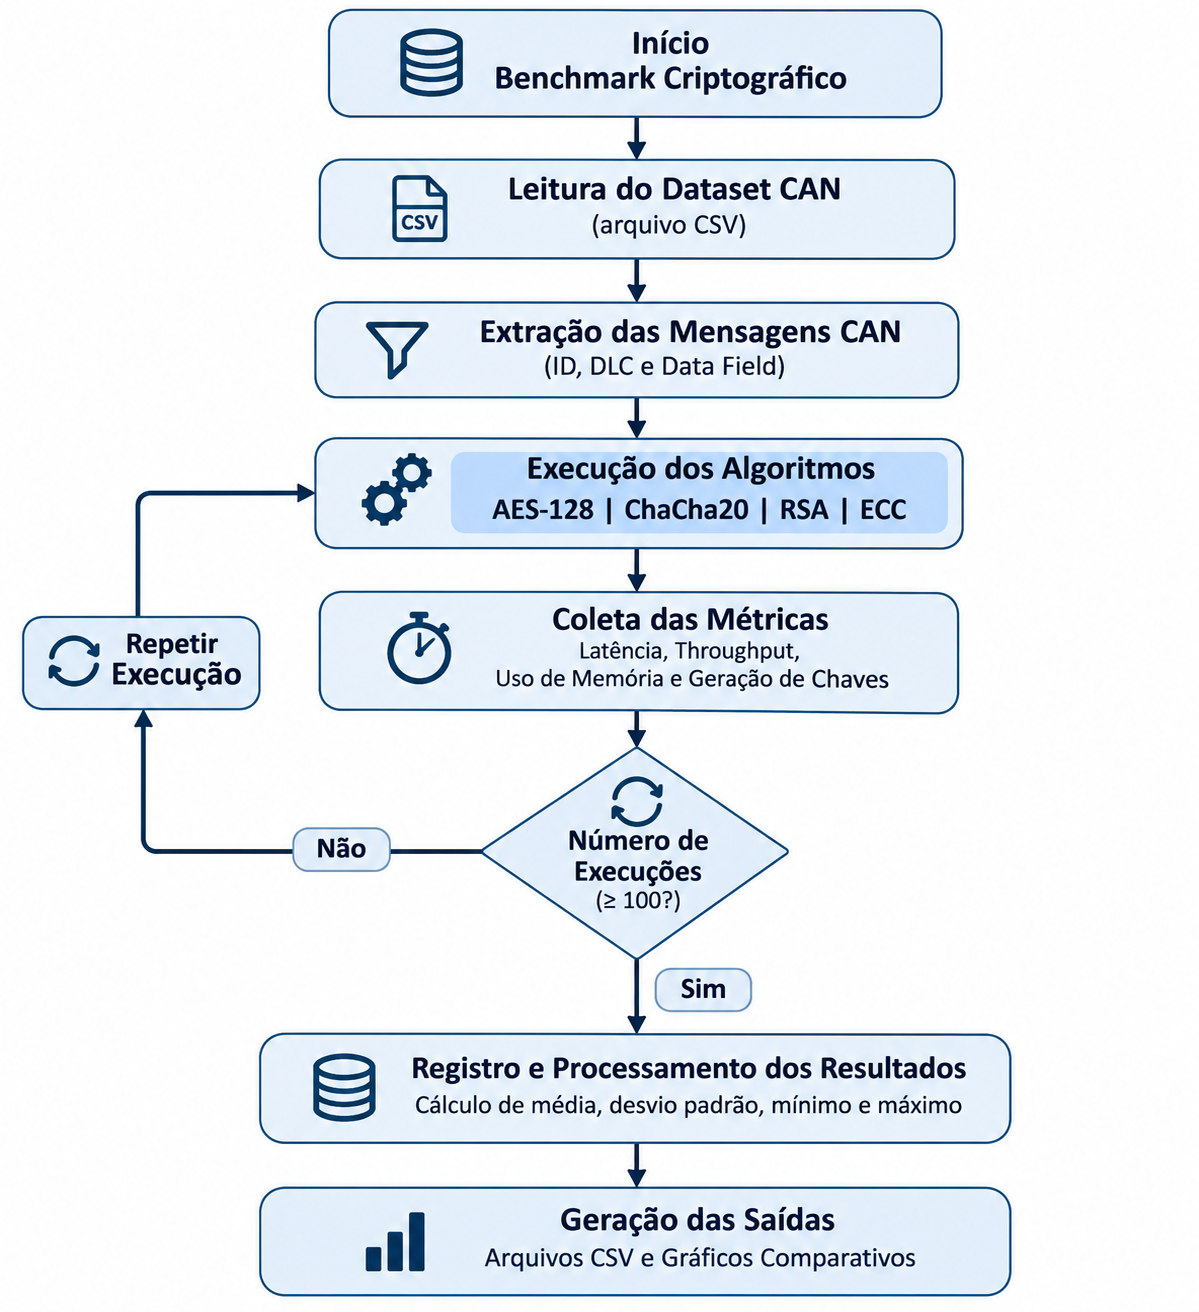
\includegraphics[width=0.83\textwidth]{images/fluxograma_benchmark.png}
    \caption{Fluxo de processamento do benchmark criptográfico com mensagens CAN}
    \label{fig:fluxograma_benchmark}
    \par\smallskip
    {\small Fonte: Elaborado pelo autor (2026).}
\end{figure}

A utilização do benchmark em computador permitiu estabelecer um ambiente de execução no qual os diferentes mecanismos criptográficos puderam ser avaliados utilizando uma mesma fonte de dados e um procedimento de coleta previamente definido. Essa organização também facilitou a repetição dos testes e o armazenamento das informações necessárias à análise posterior.

Entretanto, os resultados obtidos nessa etapa representam o desempenho das implementações em um computador convencional, utilizando a biblioteca OpenSSL e os recursos disponibilizados pelo sistema operacional Windows. Dessa forma, não devem ser interpretados diretamente como tempos de processamento de uma unidade eletrônica automotiva ou como atrasos de transmissão em um barramento CAN físico.

Essa limitação motivou a realização de uma segunda etapa experimental utilizando o microcontrolador ESP32, permitindo observar a execução dos mecanismos criptográficos em uma plataforma embarcada. Os procedimentos adotados nessa etapa são apresentados nas seções seguintes, enquanto os valores obtidos e suas respectivas comparações são discutidos no capítulo de resultados.


\section{Desenvolvimento do Benchmark no ESP32}

\begin{figure}[htbp]
    \centering
    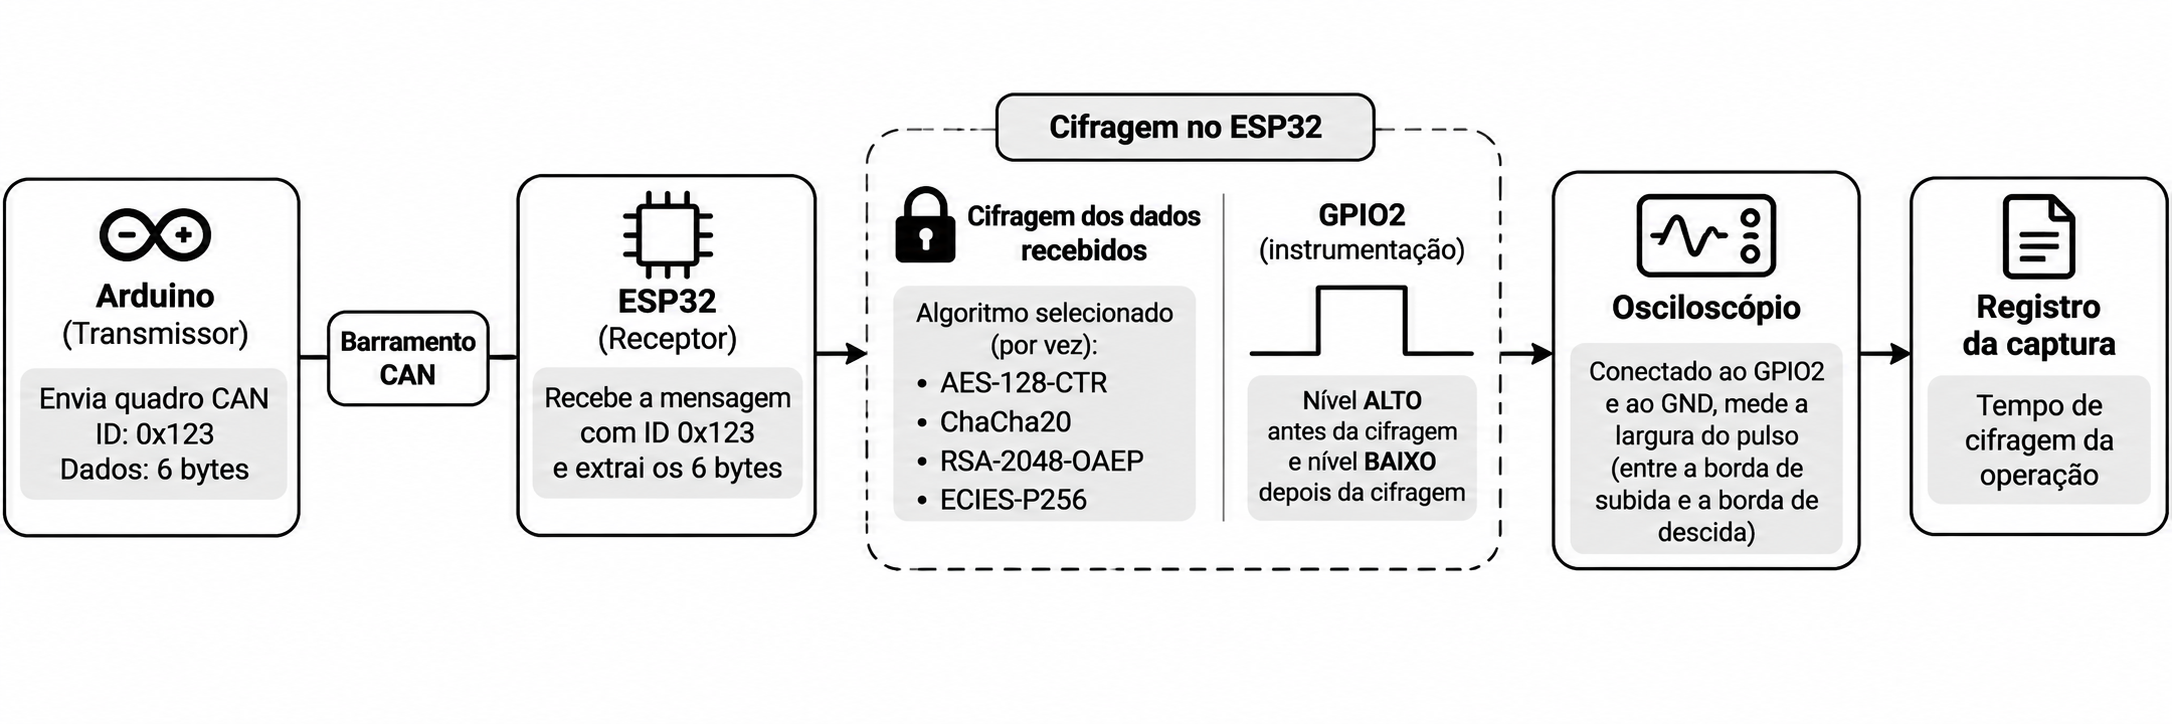
\includegraphics[width=0.83\textwidth]{images/fluxograma2.png}
    \caption{Fluxograma do procedimento experimental de medição de latência no ESP32}
    \label{fig:fluxograma-esp32}
    \fonte{Elaborado pelo autor}
\end{figure}

A segunda etapa experimental deste trabalho foi desenvolvida com o objetivo de avaliar o tempo de cifragem dos mecanismos criptográficos em uma plataforma embarcada, complementando os testes realizados anteriormente no computador. Para isso, foi utilizado um microcontrolador ESP32, responsável pelo recebimento de mensagens transmitidas por um Arduino através do barramento CAN e pela execução das operações criptográficas sobre os dados recebidos.

A utilização do ESP32 permitiu realizar os experimentos em um ambiente com características diferentes das encontradas em um computador convencional, principalmente em relação à capacidade de processamento, à disponibilidade de memória e aos recursos oferecidos pelo hardware. Essa diferença é relevante para o estudo, considerando que sistemas automotivos utilizam unidades eletrônicas embarcadas que precisam executar suas tarefas dentro de determinadas restrições temporais.

A bancada experimental foi organizada de maneira que o Arduino atuasse como dispositivo transmissor, enviando mensagens CAN com identificador hexadecimal \texttt{0x123}. O ESP32, por sua vez, foi utilizado como dispositivo receptor, responsável por identificar as mensagens recebidas e executar a rotina criptográfica correspondente ao mecanismo selecionado.

Foram considerados os mecanismos AES-128-CTR, ChaCha20, RSA-2048-OAEP e ECIES-P256. Cada mecanismo foi avaliado individualmente, permitindo observar o comportamento temporal da operação de cifragem sobre a carga útil recebida.

As mensagens utilizadas no experimento continham seis bytes de dados. A utilização de uma carga útil de tamanho constante teve como finalidade manter uniforme a quantidade de informações submetidas às operações criptográficas, evitando que diferenças no tamanho da entrada interferissem diretamente na comparação. Esse tamanho também é compatível com o limite de oito bytes de dados estabelecido para quadros CAN clássicos.

Após o recebimento da mensagem com identificador \texttt{0x123}, o ESP32 executava a operação de cifragem correspondente ao mecanismo criptográfico selecionado. O procedimento foi organizado para que o recebimento da mensagem ocorresse antes do início da medição temporal, permitindo delimitar especificamente o intervalo necessário ao processamento criptográfico.

Diferentemente de uma avaliação da comunicação completa entre os dispositivos, o experimento não teve como objetivo medir o tempo total de transmissão da mensagem pelo barramento CAN. A comunicação física foi utilizada para fornecer os dados de entrada ao ESP32, enquanto a medição temporal foi direcionada exclusivamente à região do programa responsável pela cifragem.

Dessa maneira, o experimento permitiu investigar o custo computacional dos mecanismos criptográficos em uma plataforma embarcada, utilizando mensagens recebidas de um barramento CAN físico como entrada para as operações. Os resultados dessa etapa complementam as medições realizadas no computador, permitindo discutir a influência das características de hardware e implementação sobre o desempenho dos mecanismos analisados.

\section{Instrumentação do GPIO2 e Utilização do Osciloscópio}

Para realizar a medição externa do tempo de cifragem no ESP32, foi utilizado o pino GPIO2 como sinal de referência para um osciloscópio. Essa instrumentação permitiu observar o intervalo durante o qual a rotina criptográfica estava sendo executada, utilizando as alterações de nível lógico do pino para delimitar o início e o término do processamento.

O procedimento consistiu em manter inicialmente o GPIO2 em nível lógico baixo. Após o recebimento da mensagem CAN com identificador \texttt{0x123}, o programa colocava o pino em nível lógico alto imediatamente antes da chamada da função de cifragem. Quando a operação era concluída, o GPIO2 retornava ao nível lógico baixo.

Essa sequência produzia um pulso digital cuja largura correspondia aproximadamente ao tempo necessário para executar a região de cifragem instrumentada. Dessa forma, a duração do pulso podia ser observada diretamente na tela do osciloscópio, permitindo estimar o tempo de processamento criptográfico.

A ponta de prova do osciloscópio foi conectada ao GPIO2 do ESP32, enquanto a referência de terra da sonda foi conectada ao GND da placa. Essa configuração permitiu observar as transições elétricas produzidas pelo microcontrolador durante a execução das operações.

A medição foi realizada considerando a diferença temporal entre a borda de subida e a borda de descida do pulso. A primeira transição representava o início da região de cifragem, enquanto a segunda indicava sua conclusão. O intervalo entre essas duas bordas foi utilizado como referência para estimar a latência da operação criptográfica.

Para facilitar a observação, o osciloscópio foi configurado de maneira a permitir a identificação dos níveis lógicos alto e baixo, bem como a visualização das transições do sinal. A escala horizontal foi ajustada conforme a duração dos pulsos observados, enquanto a escala vertical permitiu distinguir os níveis de tensão produzidos pelo GPIO2.

Também foi utilizado o recurso de disparo do osciloscópio, denominado \textit{trigger}, que permite sincronizar a aquisição com uma transição específica do sinal. A borda de subida do GPIO2 foi considerada como referência para o início da observação, facilitando a captura da região de processamento criptográfico.

O procedimento de instrumentação foi aplicado aos mecanismos AES-128-CTR, ChaCha20, RSA-2048-OAEP e ECIES-P256, permitindo utilizar o mesmo ponto de medição para as diferentes operações de cifragem. Dessa maneira, não foi necessário modificar a conexão física do osciloscópio ao alternar entre os mecanismos avaliados.

É importante destacar que a largura do pulso não representa exclusivamente as instruções matemáticas internas do algoritmo, pois também pode incluir pequenas parcelas relacionadas à chamada da função criptográfica e ao acionamento do próprio GPIO2. Entretanto, quando a instrumentação é mantida sob condições semelhantes, esse procedimento oferece uma referência externa para observar o tempo de processamento.

Outro aspecto relevante é que a recepção da mensagem CAN ocorre antes do acionamento do GPIO2. Portanto, o intervalo medido não inclui a arbitragem do barramento, o tempo de transmissão física do quadro ou a espera pelo recebimento da mensagem. A medição está associada especificamente à operação de cifragem realizada pelo ESP32 após a disponibilização dos dados recebidos.

Dessa forma, a utilização do GPIO2 e do osciloscópio permitiu complementar o benchmark desenvolvido em computador, fornecendo uma observação externa da duração das operações criptográficas executadas em hardware embarcado.

\section{Configuração e Validação das Capturas Experimentais}

A aquisição dos sinais foi realizada por meio de um osciloscópio conectado ao GPIO2 do ESP32. As capturas foram utilizadas para observar os pulsos digitais produzidos durante a execução das rotinas de cifragem, permitindo identificar as transições entre os níveis lógicos e os intervalos temporais delimitados pelo programa.

Para a realização das medições, foram considerados parâmetros como a escala horizontal, a escala vertical, a configuração do disparo e a posição dos cursores temporais. Esses recursos permitiram observar as formas de onda e determinar a diferença temporal entre as bordas dos pulsos.

O procedimento experimental consistiu no envio de uma mensagem CAN com identificador \texttt{0x123} pelo Arduino. Após seu recebimento, o ESP32 executava a rotina criptográfica selecionada e produzia um pulso no GPIO2 durante o processamento. O osciloscópio registrava esse sinal, permitindo visualizar a duração da operação.

A utilização de um mesmo pino de instrumentação para os diferentes mecanismos teve como finalidade manter constante o procedimento de aquisição. Assim, as diferenças observadas nas larguras dos pulsos poderiam ser relacionadas às características das rotinas executadas, desde que fossem consideradas as particularidades de cada implementação criptográfica.

A análise das capturas foi realizada considerando a identificação das bordas de subida e descida e a diferença temporal indicada pelos cursores do osciloscópio. A interpretação dos valores também levou em consideração a escala horizontal utilizada em cada aquisição, uma vez que mecanismos com diferentes custos computacionais podem exigir ajustes distintos na base de tempo do equipamento.

As capturas individuais foram utilizadas para documentar visualmente o comportamento temporal das operações criptográficas. Entretanto, uma captura isolada não permite determinar a média ou o desvio padrão de um conjunto de execuções. Para obter essas medidas estatísticas, seria necessário registrar múltiplas observações independentes de cada mecanismo e aplicar o tratamento quantitativo correspondente.

Também é importante diferenciar os registros obtidos no ambiente embarcado dos resultados do benchmark em computador. As diferenças entre processadores, bibliotecas criptográficas, otimizações e procedimentos de execução impedem que os tempos obtidos nos dois ambientes sejam considerados diretamente equivalentes.

Por fim, a validação das capturas depende da compatibilidade entre a duração indicada pelos cursores, a escala temporal configurada e a forma de onda apresentada. Somente registros que permitam identificar adequadamente o início e o término do pulso podem ser utilizados como medidas experimentais de latência.

Dessa maneira, a instrumentação por GPIO2 e a utilização do osciloscópio forneceram um procedimento para observar o tempo de cifragem dos dados recebidos pelo ESP32, complementando a análise de desempenho dos mecanismos criptográficos realizada ao longo deste trabalho.
